% Provenance (never printed): cycle 4 SVT, "La planete Terre": sedimentation,
% from sediment to sedimentary rock, fossilisation, fossils and layers as a
% record of past environments; see sources/book1/PROVENANCE.md. Book 1,
% grade 7, chapter 4.
% Vocabulary guard: first chapter allowed to use "sediment"; the principles of
% relative dating (superposition, fossil succession and the rest) and "unconformity" are
% g7.5's and are not named here; fossils as evidence of evolution are the
% biology books' (one sentence of prose).
\chapter{Sedimentos e fósseis}\label{ch:g7:sediments-and-fossils}

O Grand Canyon, no Arizona (Estados Unidos), tem em média \qty{1.6}{km}
de profundidade. As suas paredes são feitas de camadas de \omterm{def:g3:stones-pebbles-sand:rock}{rocha}, uma em
cima da outra, vermelhas, marrons, cinzentas e cor de creme. Na camada
mais alta, o Calcário Kaibab, os guardas do parque mostram conchas: as
conchas de braquiópodes, animais que viviam no fundo de um \omterm{def:g2:water-on-earth:ocean}{mar}. Essa \omterm{def:g3:stones-pebbles-sand:rock}{rocha}
se formou no fundo de um \omterm{def:g2:water-on-earth:ocean}{oceano}, e hoje forma a borda do cânion, bem acima
do \omterm{def:g4:world-physical-map:altitude}{nível do mar}.
% ledger: nps:grca-depth, nps:grca-fossils, nps:grca-kaibab

\begin{omfigure}
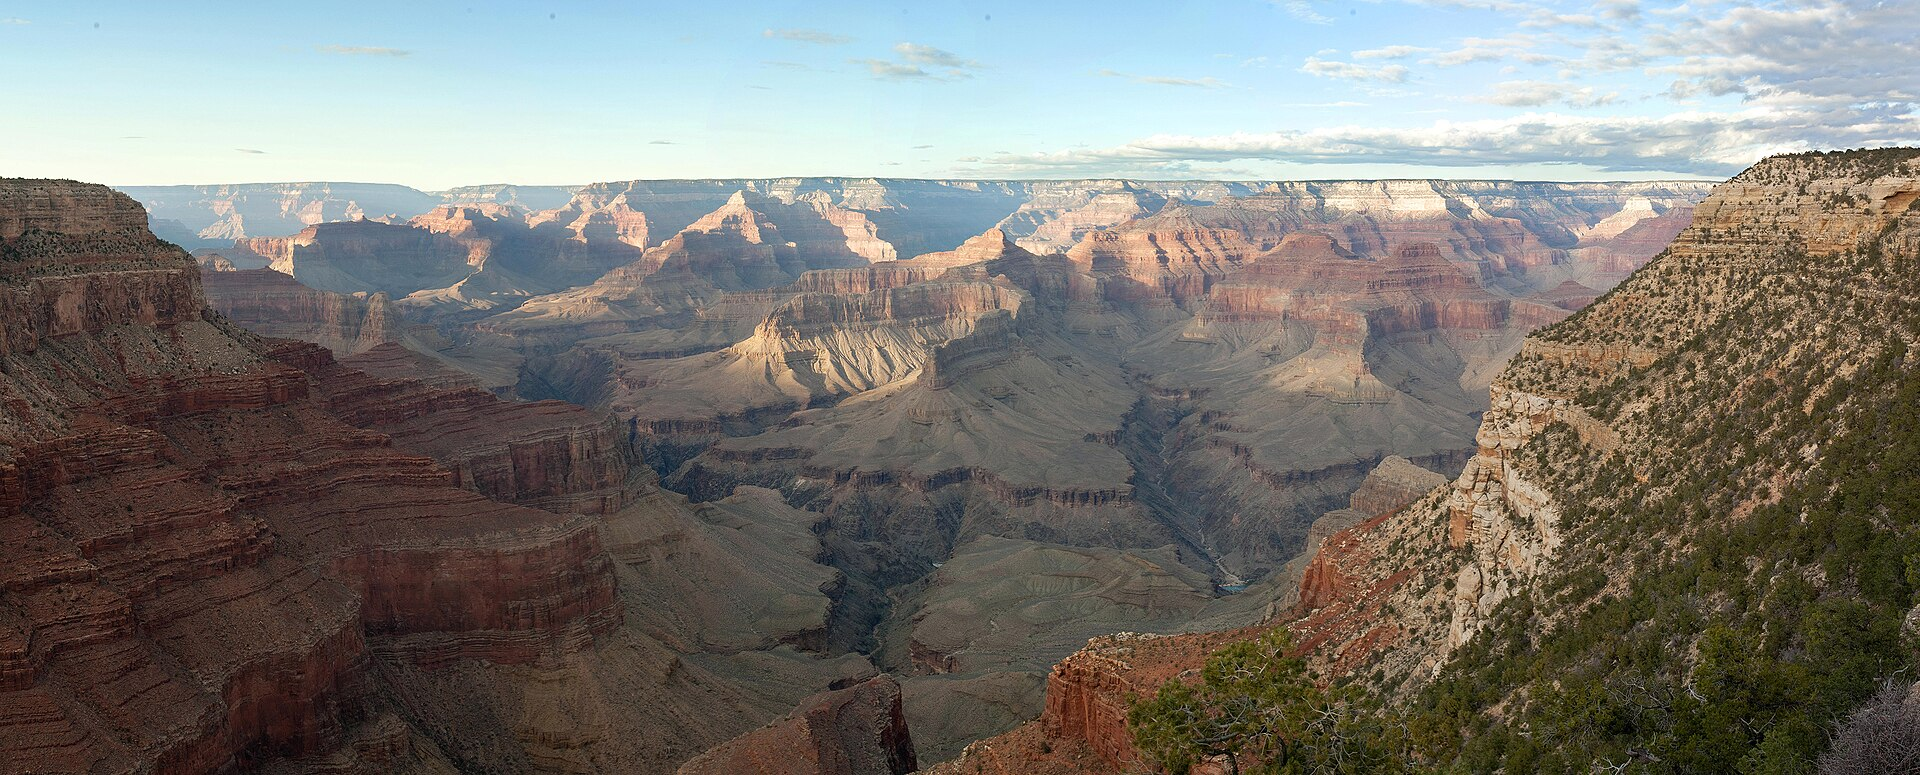
\includegraphics[width=\linewidth]{images/book1/g7-grand-canyon.jpg}

{\small O Grand Canyon visto de Hermits Rest, na sua borda sul: camada
após camada de \omterm{def:g3:stones-pebbles-sand:rock}{rocha}, da borda até o fundo. Fotografia do NPS por
Kristen M. Caldon (domínio público, via Wikimedia Commons).}
% ledger: commons:grand-canyon
\label{fig:g7:sediments-and-fossils:canyon}
\end{omfigure}

Como um monte de \omterm{def:g3:stones-pebbles-sand:sand}{areia} e de \omterm{def:g3:stones-pebbles-sand:sand}{lama} soltas vira \omterm{def:g3:stones-pebbles-sand:rock}{rocha} sólida? Como uma concha
pode durar tanto tempo que acaba dentro de um penhasco? E o que as camadas
e os \omterm{def:g7:sediments-and-fossils:fossil}{fósseis} nos contam sobre os lugares tal como eram há muito tempo?

\begin{recall}
As \omterm{def:g3:stones-pebbles-sand:rock}{rochas} são quebradas devagar em pedaços na superfície
(\emph{\omterm{def:g5:water-shapes-the-land:weathering}{intemperismo}}); a água, o vento e o gelo levam os pedaços embora
(\emph{\omterm{def:g5:water-shapes-the-land:erosion}{erosão}}) e os depositam onde eles desaceleram e param
(\emph{\omterm{def:g5:water-shapes-the-land:deposition}{deposição}}): os mais pesados primeiro, a \omterm{def:g3:stones-pebbles-sand:sand}{lama} fina só onde a água
está quase parada (\cref{ch:g5:water-shapes-the-land}). Uma \emph{\omterm{def:g6:rocks-and-minerals:rock-families}{rocha
sedimentar}} se forma na superfície a partir de grãos de \omterm{def:g3:stones-pebbles-sand:sand}{areia} e de \omterm{def:g3:stones-pebbles-sand:sand}{lama},
ou de conchas, depositados em camadas e endurecidos: arenito, folhelho,
calcário. O \omterm{def:g6:rocks-and-minerals:rock-cycle}{ciclo das rochas} transforma devagar as \omterm{def:g3:stones-pebbles-sand:rock}{rochas} de cada família
nas das outras (\cref{ch:g6:rocks-and-minerals}).
\end{recall}

\section{Os sedimentos se depositam em camadas}

Onde quer que a água, o vento ou o gelo larguem o que carregavam, um
depósito solto se acumula: \omterm{def:g3:stones-pebbles-sand:pebble}{cascalho} e \omterm{def:g3:stones-pebbles-sand:sand}{areia} no leito de um \omterm{def:g1:landscapes-around-us:water}{rio}, \omterm{def:g3:stones-pebbles-sand:sand}{lama} no
fundo de um \omterm{def:g1:landscapes-around-us:water}{lago}, \omterm{def:g3:stones-pebbles-sand:sand}{areia} numa praia ou numa duna, conchas no fundo do \omterm{def:g2:water-on-earth:ocean}{mar}.

\begin{definition}[Sedimento]\label{def:g7:sediments-and-fossils:sediment}
Um \emph{sedimento}\index{sedimento} é um material solto depositado pela
água, pelo vento ou pelo gelo: \omterm{def:g3:stones-pebbles-sand:pebble}{cascalho}, \omterm{def:g3:stones-pebbles-sand:sand}{areia}, \omterm{def:g3:stones-pebbles-sand:sand}{lama}, ou as conchas e os
esqueletos de seres vivos. Ele se acumula no fundo dos \omterm{def:g1:landscapes-around-us:water}{rios}, dos \omterm{def:g1:landscapes-around-us:water}{lagos} e
dos \omterm{def:g2:water-on-earth:ocean}{mares}, e em terra, onde o vento ou o gelo o larga.
\end{definition}

Os \omterm{def:g7:sediments-and-fossils:sediment}{sedimentos} se depositam numa ordem certa. Quando a água barrenta
desacelera, os grãos maiores e mais pesados afundam primeiro, e os menores
e mais leves por último. Cada vez que a água muda --- uma enchente que
traz \omterm{def:g3:stones-pebbles-sand:sand}{areia}, e depois semanas calmas em que só a \omterm{def:g3:stones-pebbles-sand:sand}{lama} fina chega ao fundo
---, os grãos que se depositam também mudam, e uma nova camada começa.
Pouco a pouco, o fundo de um \omterm{def:g1:landscapes-around-us:water}{lago} ou de um \omterm{def:g2:water-on-earth:ocean}{mar} se cobre de uma pilha de
camadas, as mais velhas embaixo da pilha.
% ledger: usgs:strata, usgs:sediments-to-rock

\begin{omfigure}
\begin{tikzpicture}[font=\small, x=1cm, y=1cm]
  % land and river
  \fill[omLithAlluv] (0,3.0) -- (2.0,2.45) -- (2.0,0) -- (0,0) -- cycle;
  \fill[blue!35] (0,3.05) -- (2.0,2.5) -- (2.0,2.4) -- (0,2.95) -- cycle;
  % lake water
  \fill[omSea!45] (2.0,2.5) -- (12.4,2.5) -- (12.4,1.12) -- (3.0,1.2) -- cycle;
  \draw[blue!50!black, line width=0.6pt] (2.0,2.5) -- (12.4,2.5);
  % layers on the bottom: thick near the mouth, thinner far out
  \foreach \k/\c in {0/omLithSand, 1/omLithShale, 2/omLithSand, 3/omLithShale} {
    \pgfmathsetmacro{\yb}{0.2+0.25*\k}
    \pgfmathsetmacro{\yt}{0.2+0.25*(\k+1)}
    \fill[\c] (3.0,\yb) -- (12.4,\yb) -- (12.4,\yt-0.08) -- (3.0,\yt) -- cycle;
  }
  \draw[black!60, line width=0.3pt] (3.0,1.2) -- (12.4,1.12);
  \fill[omLithAlluv!80!black] (2.0,0) rectangle (12.4,0.2);
  \fill[omLithAlluv] (2.0,0.2) -- (3.0,0.2) -- (3.0,1.2) -- (2.0,2.45) -- cycle;
  % settling grains: big ones near the mouth, fine ones far out
  \foreach \x/\y in {3.3/2.1, 3.6/1.75, 3.9/2.25, 4.2/1.55, 3.5/1.35, 4.5/2.0} {
    \fill[brown!70!black] (\x,\y) circle (0.07);
    \draw[-{Stealth[length=1.3mm]}, black!60] (\x,\y-0.1) -- (\x,\y-0.32);
  }
  \foreach \x/\y in {6.5/2.2, 7.4/1.8, 8.3/2.15, 9.1/1.6, 9.9/2.05, 10.8/1.75, 11.6/2.1, 7.9/1.35, 10.4/1.3} {
    \fill[brown!50!black] (\x,\y) circle (0.025);
    \draw[-{Stealth[length=1mm]}, black!40] (\x,\y-0.05) -- (\x,\y-0.2);
  }
  \node[anchor=south, align=center] at (1.0,3.1) {um rio na cheia\\[-2pt]traz areia e lama};
  \node[anchor=south, align=center] at (4.1,2.55) {a areia se deposita\\[-2pt]primeiro, perto da foz};
  \node[anchor=south, align=center] at (9.2,2.55) {a lama fina se deposita devagar,\\[-2pt]mais longe, onde a água está calma};
  \draw[decorate, decoration={brace, amplitude=4pt}] (12.55,1.15) -- (12.55,0.2)
    node[midway, anchor=west, xshift=4pt, align=left, font=\footnotesize] {camadas no\\[-2pt]fundo: areia,\\[-2pt]lama, areia, lama};
\end{tikzpicture}

{\small \omterm{def:g7:sediments-and-fossils:sediment}{Sedimentos} se depositando num \omterm{def:g1:landscapes-around-us:water}{lago} (um desenho, fora de escala).
Depois de cada cheia, uma camada de \omterm{def:g3:stones-pebbles-sand:sand}{areia} se deposita, e depois a \omterm{def:g3:stones-pebbles-sand:sand}{lama}
fina nas semanas calmas que vêm em seguida: camada após camada, o fundo
vai se cobrindo.}
% ledger: usgs:strata
\label{fig:g7:sediments-and-fossils:lake}
\end{omfigure}

\begin{definition}[Camada sedimentar]\label{def:g7:sediments-and-fossils:layer}
Uma \emph{camada sedimentar}\index{camada sedimentar}, ou
\emph{estrato}\index{estrato (camada)} (plural \emph{estratos}), é uma lâmina de
\omterm{def:g7:sediments-and-fossils:sediment}{sedimento}, ou da \omterm{def:g3:stones-pebbles-sand:rock}{rocha} em que ele se transformou, depositada de uma só
vez. Ela tem uma base e um topo, e se distingue das camadas de cima e de
baixo pelo tamanho dos seus grãos ou por aquilo de que é feita.
\end{definition}

Os \omterm{def:g7:sediments-and-fossils:sediment}{sedimentos} se depositam a partir da água ou do ar, então eles ficam
deitados na horizontal, como as páginas de um livro em cima de uma mesa.
Quando encontramos camadas inclinadas ou dobradas, algo as moveu depois
que elas se formaram. As camadas são a marca mais clara de uma \omterm{def:g6:rocks-and-minerals:rock-families}{rocha
sedimentar}: você as viu nas paredes do Grand Canyon.
% ledger: usgs:strata, nps:grca-kaibab

\begin{inthelab}[Camadas num pote (em aula, com a professora)]
Ponha um punhado de \omterm{def:g3:stones-pebbles-sand:pebble}{cascalho}, dois punhados de \omterm{def:g3:stones-pebbles-sand:sand}{areia} e algumas colheradas
de terra num pote de vidro alto; encha-o de água, feche-o bem e sacuda-o.
Ponha o pote na mesa e observe durante alguns minutos: o \omterm{def:g3:stones-pebbles-sand:pebble}{cascalho} chega
ao fundo na hora, a \omterm{def:g3:stones-pebbles-sand:sand}{areia} um pouco depois, e a \omterm{def:g3:stones-pebbles-sand:sand}{lama} fina deixa a água
turva durante horas. No dia seguinte, acrescente um pouco mais de terra e
de \omterm{def:g3:stones-pebbles-sand:sand}{areia}, sacuda de leve e deixe assentar de novo. Quantas camadas você
consegue contar? Que grãos ficam embaixo de cada uma?
\end{inthelab}

\section{Do sedimento à rocha}

Uma camada não fica muito tempo por cima. Outras camadas se depositam
sobre ela, e depois outras, e ela vai ficando enterrada cada vez mais
fundo. Sob o peso das camadas de cima, os grãos são apertados uns contra
os outros e a água entre eles é espremida para fora. A água que se
infiltra pela pilha deixa \omterm{def:g6:rocks-and-minerals:mineral}{minerais} entre os grãos, um cimento natural que
os gruda uns nos outros. Com muito tempo, com mais camadas se empilhando
e lentas mudanças químicas, o \omterm{def:g7:sediments-and-fossils:sediment}{sedimento} solto do fundo da pilha vira
\omterm{def:g3:stones-pebbles-sand:rock}{rocha}.
% ledger: usgs:sediments-to-rock, usgs:sedimentary

Cada tipo de \omterm{def:g7:sediments-and-fossils:sediment}{sedimento} dá a sua própria \omterm{def:g3:stones-pebbles-sand:rock}{rocha}.

\begin{center}
\small
\begin{tabular}{|l|l|}
\hline
\textbf{\omterm{def:g7:sediments-and-fossils:sediment}{sedimento}} & \textbf{a \omterm{def:g3:stones-pebbles-sand:rock}{rocha} em que ele se transforma} \\
\hline
\omterm{def:g3:stones-pebbles-sand:pebble}{cascalho} e \omterm{def:g3:stones-pebbles-sand:pebble}{seixos} & conglomerado \\
\omterm{def:g3:stones-pebbles-sand:sand}{areia} & arenito \\
\omterm{def:g3:stones-pebbles-sand:sand}{lama} & lamito, ou folhelho quando ele se parte em lâminas finas \\
conchas e esqueletos & calcário \\
restos de plantas, enterrados num pântano & carvão \\
\hline
\end{tabular}
\end{center}
% ledger: usgs:sediments-to-rock, usgs:sedimentary, usgs:coal-origin

\begin{omfigure}
\begin{tikzpicture}[font=\small, x=1cm, y=1cm]
  \pgfmathsetseed{11}
  \foreach \p/\gap/\title in {0/0.40/{sedimento solto}, 1/0.31/{enterrado e apertado:\\[-2pt]a água sai}, 2/0.31/{cimentado: uma rocha}} {
    \begin{scope}[xshift=\p*4.6cm]
      \ifnum\p=2 \fill[black!25] (0,0) rectangle (3.4,3.0);
      \else \fill[omSea!45] (0,0) rectangle (3.4,3.0); \fi
      \foreach \i in {0,...,7} {
        \foreach \j in {0,...,6} {
          \pgfmathsetmacro{\gx}{0.25 + \i*\gap*1.05 + 0.05*rand}
          \pgfmathsetmacro{\gy}{0.25 + \j*\gap + 0.05*rand}
          \pgfmathsetmacro{\gr}{0.13 + 0.03*rand}
          \ifdim\gx pt<3.25pt \ifdim\gy pt<2.85pt
            \fill[omLithSand!80!brown, draw=brown!60!black, line width=0.3pt] (\gx,\gy) circle (\gr);
          \fi\fi
        }
      }
      \draw[black!70, line width=0.6pt] (0,0) rectangle (3.4,3.0);
      \node[anchor=north, align=center] at (1.7,-0.1) {\title};
    \end{scope}
  }
  \draw[-{Stealth[length=2.5mm]}, line width=1pt] (3.6,1.5) -- (4.4,1.5);
  \draw[-{Stealth[length=2.5mm]}, line width=1pt] (8.2,1.5) -- (9.0,1.5);
  \foreach \x in {5.3,6.3,7.3} \draw[-{Stealth[length=2mm]}, line width=0.8pt] (\x,3.7) -- (\x,3.1);
  \node[anchor=south] at (6.3,3.7) {peso das camadas de cima};
  \node[anchor=south, font=\footnotesize, align=center] at (10.9,3.05) {cinza: o cimento natural};
\end{tikzpicture}

{\small Da \omterm{def:g3:stones-pebbles-sand:sand}{areia} ao arenito (um desenho dos grãos, muito aumentados). À
esquerda: grãos soltos, com água entre eles. No meio: enterrados embaixo
de novas camadas, os grãos são apertados uns contra os outros. À direita:
os \omterm{def:g6:rocks-and-minerals:mineral}{minerais} deixados pela água grudam os grãos uns nos outros.}
% ledger: usgs:sediments-to-rock, usgs:sedimentary
\label{fig:g7:sediments-and-fossils:to-rock}
\end{omfigure}

A maior parte das \omterm{def:g3:stones-pebbles-sand:rock}{rochas} que você vê na superfície da Terra é
sedimentar. A pilha de camadas que elas formam é o livro de história do
lugar: cada camada é uma página, e as páginas mais velhas ficam embaixo.
% ledger: usgs:sediments-to-rock

\section{Como se forma um fóssil}

\begin{definition}[Fóssil]\label{def:g7:sediments-and-fossils:fossil}
Um \emph{fóssil}\index{fossil@fóssil} é o resto, ou o vestígio, de um ser
vivo de muito tempo atrás, conservado na \omterm{def:g3:stones-pebbles-sand:rock}{rocha}. Alguns fósseis são as
partes duras do corpo --- uma concha, um osso, um dente, madeira ---
transformadas em pedra. Outros guardam só uma forma: um
\emph{molde}\index{molde} é a marca oca deixada na \omterm{def:g3:stones-pebbles-sand:rock}{rocha} onde uma concha
ou um osso se dissolveu; um \emph{contramolde}\index{contramolde} é a
cópia que se forma quando um molde se enche de nova matéria \omterm{def:g6:rocks-and-minerals:mineral}{mineral} ou de
\omterm{def:g7:sediments-and-fossils:sediment}{sedimento}. Um \emph{icnofóssil}\index{icnofossil@icnofóssil} é um sinal
do que um animal fez --- uma pegada, uma toca, um rastro --- e não uma
parte do seu corpo.
\end{definition}

Um \omterm{def:g7:sediments-and-fossils:fossil}{fóssil} começa a sua vida como um animal ou uma planta morta no fundo
de um \omterm{def:g2:water-on-earth:ocean}{mar} ou de um \omterm{def:g1:landscapes-around-us:water}{lago}. Se ele fica descoberto, as bactérias o
decompõem, e a água dissolve devagar o que sobra. Ele só tem chance se
for enterrado depressa, embaixo de um \omterm{def:g7:sediments-and-fossils:sediment}{sedimento} que se deposita sobre ele
e o isola. Depois, enquanto o \omterm{def:g7:sediments-and-fossils:sediment}{sedimento} vira \omterm{def:g3:stones-pebbles-sand:rock}{rocha}, a água que se
infiltra pelas camadas traz \omterm{def:g6:rocks-and-minerals:mineral}{minerais} que preenchem cada buraquinho da
concha ou do osso: ele vira pedra. Muito tempo depois, as camadas de cima
podem ser desgastadas, e o \omterm{def:g7:sediments-and-fossils:fossil}{fóssil} aparece na superfície.
% ledger: ucmp:fossil-conditions, ucmp:fossil-kinds, usgs:sediments-to-rock

\begin{omfigure}
\begin{tikzpicture}[font=\small, x=0.86cm, y=0.86cm,
    shell/.pic={
      \fill[#1] (0,0) circle (0.42);
      \draw[brown!40!black, line width=0.5pt] plot[domain=0:12.5, samples=90, smooth]
        ({0.032*\x*cos(\x r)}, {0.032*\x*sin(\x r)});
      \draw[brown!40!black, line width=0.5pt] (0,0) circle (0.42);
    }]
  % 1: death on the sea floor
  \begin{scope}[xshift=0cm]
    \fill[omSea!45] (0,1.2) rectangle (3.3,3.6);
    \fill[omLithShale] (0,0) rectangle (3.3,1.2);
    \pic at (1.65,1.62) {shell=omLithSand!60!white};
    \node[anchor=north, align=center] at (1.65,-0.1) {1. ele morre no\\[-2pt]fundo do mar};
  \end{scope}
  % 2: quick burial
  \begin{scope}[xshift=3.75cm]
    \fill[omSea!45] (0,2.1) rectangle (3.3,3.6);
    \fill[omLithShale] (0,0) rectangle (3.3,1.2);
    \fill[omLithShale!70!white] (0,1.2) rectangle (3.3,2.1);
    \pic at (1.65,1.62) {shell=omLithSand!60!white};
    \foreach \x in {0.5,1.2,2.1,2.8} \fill[brown!50!black] (\x,2.4) circle (0.03);
    \node[anchor=north, align=center] at (1.65,-0.1) {2. a lama o cobre\\[-2pt]depressa};
  \end{scope}
  % 3: buried deep, turned to stone
  \begin{scope}[xshift=7.5cm]
    \fill[omLithShale!80!black] (0,0) rectangle (3.3,1.2);
    \fill[omLithShale!85!black] (0,1.2) rectangle (3.3,2.1);
    \fill[omLithSand] (0,2.1) rectangle (3.3,2.9);
    \fill[omLithLime] (0,2.9) rectangle (3.3,3.6);
    \pic at (1.65,1.62) {shell=black!35};
    \node[anchor=north, align=center] at (1.65,-0.1) {3. enterrado fundo,\\[-2pt]ele vira pedra};
  \end{scope}
  % 4: uncovered by erosion
  \begin{scope}[xshift=11.25cm]
    \fill[white] (0,0) rectangle (3.3,3.6);
    \fill[omLithShale!80!black] (0,0) -- (3.3,0) -- (3.3,2.6) -- (2.4,2.3) -- (1.8,1.95) -- (1.2,1.7) -- (0,1.5) -- cycle;
    \draw[black!35, line width=0.4pt] (0,1.2) -- (3.3,1.2);
    \draw[black!60, line width=0.4pt] (0,1.5) -- (1.2,1.7) -- (1.8,1.95) -- (2.4,2.3) -- (3.3,2.6);
    \pic at (1.65,1.84) {shell=black!35};
    \node[anchor=north, align=center] at (1.65,-0.1) {4. a erosão o traz\\[-2pt]para a superfície};
  \end{scope}
  \foreach \p in {0,1,2,3} {
    \begin{scope}[xshift=\p*3.75cm]
      \draw[black!70, line width=0.5pt] (0,0) rectangle (3.3,3.6);
    \end{scope}
  }
\end{tikzpicture}

{\small Como se forma um \omterm{def:g7:sediments-and-fossils:fossil}{fóssil} (um desenho, fora de escala): uma concha é
enterrada depressa embaixo da \omterm{def:g3:stones-pebbles-sand:sand}{lama}; enterrada mais fundo embaixo de novas
camadas, ela vira pedra; muito tempo depois, a \omterm{def:g5:water-shapes-the-land:erosion}{erosão} desgasta as camadas
de cima e o \omterm{def:g7:sediments-and-fossils:fossil}{fóssil} aparece na superfície.}
% ledger: ucmp:fossil-conditions, ucmp:fossil-kinds
\label{fig:g7:sediments-and-fossils:steps}
\end{omfigure}

A maioria dos seres vivos não deixa nenhum \omterm{def:g7:sediments-and-fossils:fossil}{fóssil}. Os corpos moles
apodrecem antes de poderem ser enterrados; até as conchas e os ossos se
quebram ou se dissolvem se ficam muito tempo descobertos. O melhor lugar
para virar \omterm{def:g7:sediments-and-fossils:fossil}{fóssil} é o fundo de um \omterm{def:g2:water-on-earth:ocean}{mar} ou de um \omterm{def:g1:landscapes-around-us:water}{lago} tranquilo, onde a
\omterm{def:g3:stones-pebbles-sand:sand}{lama} fina se deposita sobre os restos e os protege. É por isso que os
\omterm{def:g7:sediments-and-fossils:fossil}{fósseis} encontrados nas \omterm{def:g3:stones-pebbles-sand:rock}{rochas} são sobretudo conchas, e as conchinhas e
os restos de plantas e animais microscópicos; os dinossauros, os \omterm{def:g7:sediments-and-fossils:fossil}{fósseis}
mais famosos, são só uma parte muito pequena deles.
% ledger: ucmp:fossil-conditions, usgs:fossil-record-shells

\begin{omfigure}
\begin{minipage}[t]{0.49\linewidth}\centering
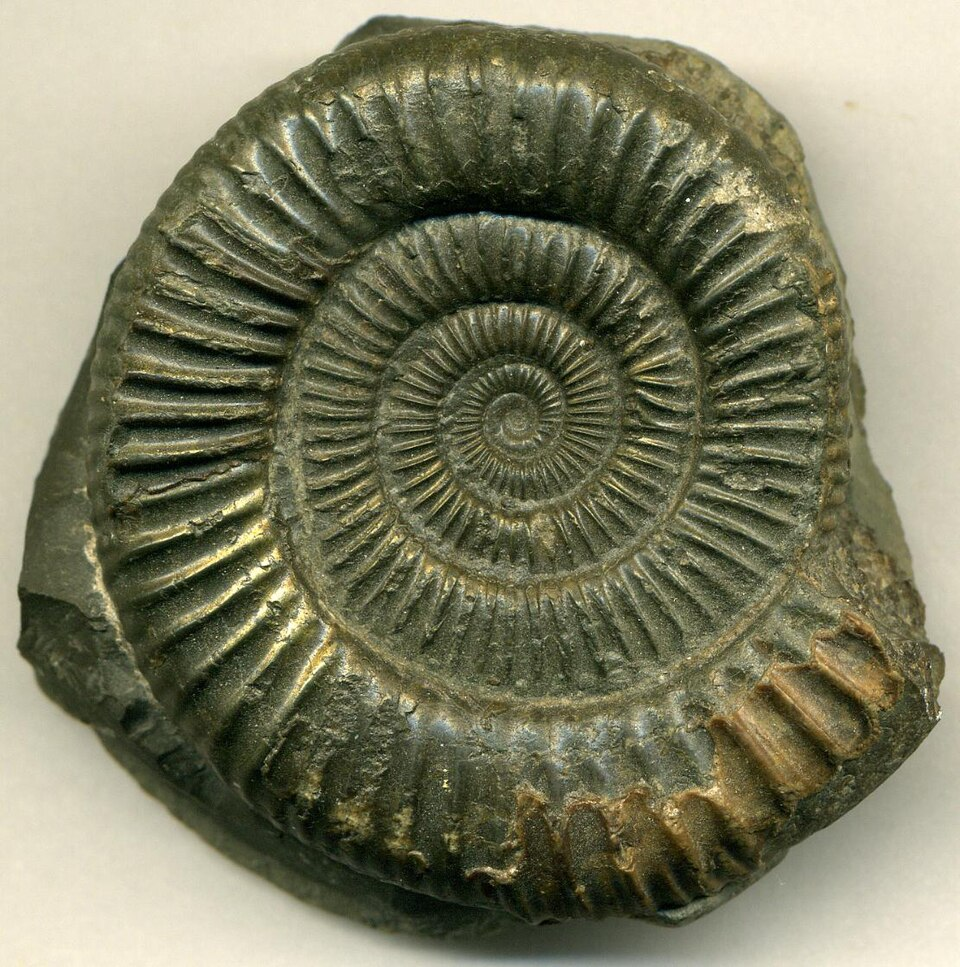
\includegraphics[height=4.6cm]{images/book1/g7-ammonite.jpg}

{\small Uma amonite, um animal extinto de concha enrolada, parente das
lulas e dos polvos, com \qty{5.7}{cm} de diâmetro, do \omterm{def:g1:landscapes-around-us:water}{litoral} de
Yorkshire (Inglaterra).}
\end{minipage}\hfill
\begin{minipage}[t]{0.49\linewidth}\centering
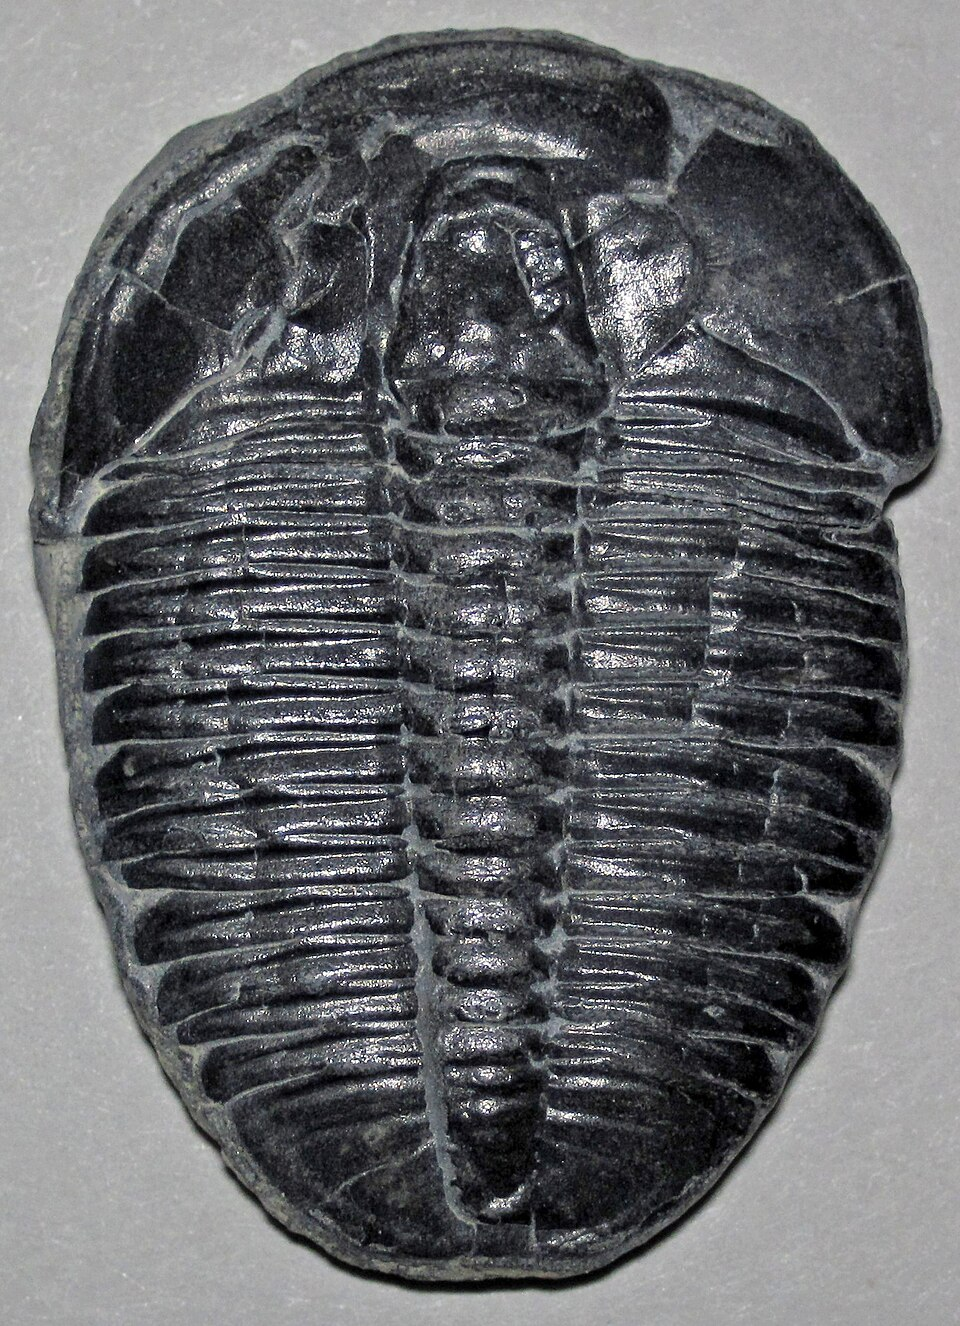
\includegraphics[height=4.6cm]{images/book1/g7-trilobite.jpg}

{\small Um trilobita, um animal marinho extinto cujo corpo tem três lobos,
com cerca de \qty{2.6}{cm} de largura, de Utah (Estados Unidos).}
\end{minipage}\par\medskip

{\small Dois \omterm{def:g7:sediments-and-fossils:fossil}{fósseis} de animais de concha dura. Fotografias: James
St.~John (CC BY 2.0, via Wikimedia Commons).}
% ledger: commons:ammonite, commons:trilobite, nps:ammonoid, nps:trilobite
\label{fig:g7:sediments-and-fossils:ammonite-trilobite}
\end{omfigure}

Às vezes, a própria concha não dura. Enterrada na \omterm{def:g3:stones-pebbles-sand:sand}{areia}, ela é dissolvida
devagar pela água que se infiltra entre os grãos, e só sobra um oco, com
a forma da concha impressa nas suas paredes: um \omterm{def:g7:sediments-and-fossils:fossil}{molde}. Se depois \omterm{def:g6:rocks-and-minerals:mineral}{minerais}
se depositam no oco e o preenchem, eles fazem uma cópia da concha: um
\omterm{def:g7:sediments-and-fossils:fossil}{contramolde}.
% ledger: ucmp:casts-molds

\begin{omfigure}
\begin{tikzpicture}[font=\small, x=1cm, y=1cm,
    clam/.style={line width=0.5pt}]
  \foreach \p/\fillc/\title in {0/{omLithSand!50!white}/{uma concha enterrada\\[-2pt]na areia}, 1/{white}/{a concha se dissolveu:\\[-2pt]um molde}, 2/{black!40}/{minerais preenchem o molde:\\[-2pt]um contramolde}} {
    \begin{scope}[xshift=\p*4.9cm]
      \fill[omLithSand] (0,0) rectangle (4.2,2.6);
      \foreach \i in {0,...,40} {
        \pgfmathsetmacro{\gx}{0.1+mod(\i*0.53,4.0)}
        \pgfmathsetmacro{\gy}{0.1+mod(\i*0.37,2.4)}
        \fill[brown!60!black] (\gx,\gy) circle (0.025);
      }
      \fill[\fillc, draw=brown!40!black, clam] (0.9,0.9) arc[start angle=180, end angle=0, x radius=1.2, y radius=0.95] -- cycle;
      \ifnum\p=1
        \foreach \a in {25,45,...,155} \draw[brown!50!black, line width=0.4pt] (2.1,0.9) -- ++(\a:0.93 and 0.75);
      \else
        \foreach \a in {25,45,...,155} \draw[brown!40!black, line width=0.4pt] (2.1,0.9) -- ++(\a:1.05 and 0.85);
      \fi
      \draw[black!70, line width=0.5pt] (0,0) rectangle (4.2,2.6);
      \node[anchor=north, align=center] at (2.1,-0.1) {\title};
    \end{scope}
  }
  \draw[-{Stealth[length=2.5mm]}, line width=1pt] (4.3,1.3) -- (4.8,1.3);
  \draw[-{Stealth[length=2.5mm]}, line width=1pt] (9.2,1.3) -- (9.7,1.3);
\end{tikzpicture}

{\small Um \omterm{def:g7:sediments-and-fossils:fossil}{molde} e um \omterm{def:g7:sediments-and-fossils:fossil}{contramolde} (um desenho, num corte da \omterm{def:g3:stones-pebbles-sand:rock}{rocha}). O
\omterm{def:g7:sediments-and-fossils:fossil}{molde} é o oco, com as nervuras da concha impressas na sua parede; o
\omterm{def:g7:sediments-and-fossils:fossil}{contramolde} é uma cópia de pedra da concha, feita dos \omterm{def:g6:rocks-and-minerals:mineral}{minerais} que o
preencheram.}
% ledger: ucmp:casts-molds
\label{fig:g7:sediments-and-fossils:mould-cast}
\end{omfigure}

Os animais também deixam \omterm{def:g7:sediments-and-fossils:fossil}{fósseis} do que eles fizeram. Um animal que anda
na \omterm{def:g3:stones-pebbles-sand:sand}{lama} mole e molhada da margem de um \omterm{def:g1:landscapes-around-us:water}{rio} ou de uma praia deixa pegadas.
A maioria é apagada pela onda seguinte ou pela cheia seguinte. Mas, se a
\omterm{def:g3:stones-pebbles-sand:sand}{areia} as cobre antes de serem apagadas, a pegada é preenchida, a \omterm{def:g3:stones-pebbles-sand:sand}{areia}
depois vira arenito, e, quando a \omterm{def:g3:stones-pebbles-sand:rock}{rocha} se parte ao longo da camada, ela
mostra a pegada e, do outro lado, o seu \omterm{def:g7:sediments-and-fossils:fossil}{contramolde}.
% ledger: ucmp:footprints

\begin{omfigure}
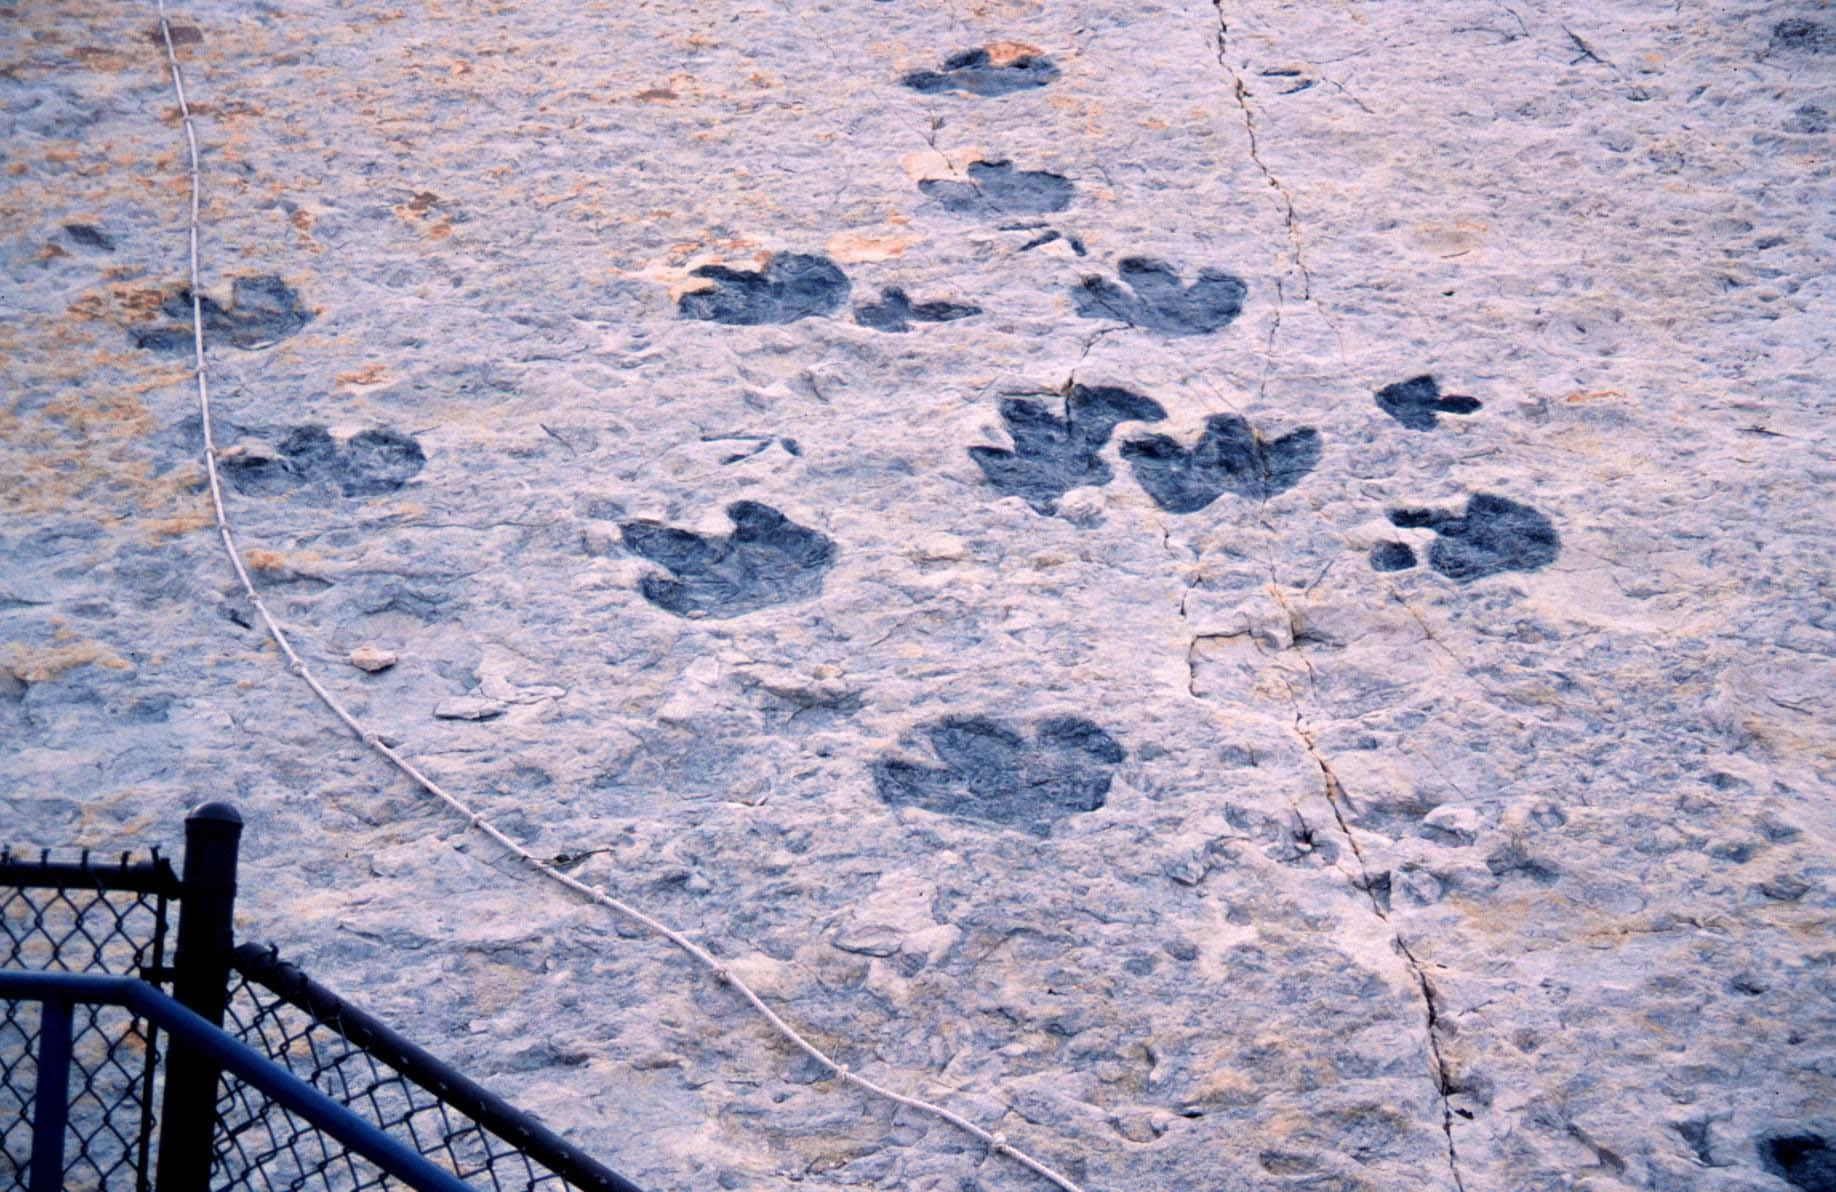
\includegraphics[width=0.62\linewidth]{images/book1/g7-dinosaur-tracks.jpg}

{\small Pegadas de dinossauros em Dinosaur Ridge, perto de Morrison, no
Colorado (Estados Unidos): dezenas de pegadas deixadas num chão mole, que
hoje é uma superfície de \omterm{def:g3:stones-pebbles-sand:rock}{rocha} inclinada. A maioria foi feita por
dinossauros que comiam plantas, algumas por carnívoros de dedos finos.
Fotografia: Dexter Perkins (CC0, via Wikimedia Commons).}
% ledger: commons:dino-tracks
\label{fig:g7:sediments-and-fossils:tracks}
\end{omfigure}

A biologia usa os \omterm{def:g7:sediments-and-fossils:fossil}{fósseis} para acompanhar a longa história dos seres
vivos. Neste livro, os \omterm{def:g7:sediments-and-fossils:fossil}{fósseis} são pistas de outro tipo: eles nos contam
como era o lugar quando o animal vivia ali.

\section{Camadas e fósseis, um registro do passado}

Cada camada guarda as marcas do lugar onde foi depositada. Os recifes de
coral crescem hoje em \omterm{def:g2:water-on-earth:ocean}{mares} quentes, claros e rasos; as marcas de
ondulação se formam na \omterm{def:g3:stones-pebbles-sand:sand}{areia} em águas rasas, na beira de um \omterm{def:g1:landscapes-around-us:water}{lago}, de um
\omterm{def:g1:landscapes-around-us:water}{rio} ou de um \omterm{def:g2:water-on-earth:ocean}{mar}; o carvão se formou a partir das plantas de antigas
florestas e brejos; os braquiópodes, os crinoides e os trilobitas viviam só no \omterm{def:g2:water-on-earth:ocean}{mar}. Quando as mesmas pistas são encontradas numa camada antiga, o lugar
provavelmente era assim quando a camada se formou.
% ledger: noaa:coral-where, nps:ripple-marks, nps:ripples-shallow, usgs:coal-origin, nps:trilobite

\begin{center}
\small
\begin{tabular}{|p{0.36\linewidth}|p{0.52\linewidth}|}
\hline
\textbf{pista na camada} & \textbf{o lugar quando a camada se formou} \\
\hline
corais & um \omterm{def:g2:water-on-earth:ocean}{mar} quente, raso e claro \\
\hline
conchas de animais marinhos (braquiópodes, crinoides, trilobitas) & um \omterm{def:g2:water-on-earth:ocean}{mar} \\
\hline
marcas de ondulação na superfície de uma camada & águas rasas, na beira de um \omterm{def:g1:landscapes-around-us:water}{lago}, de um \omterm{def:g1:landscapes-around-us:water}{rio} ou de um \omterm{def:g2:water-on-earth:ocean}{mar} \\
\hline
pegadas & \omterm{def:g3:stones-pebbles-sand:sand}{lama} ou \omterm{def:g3:stones-pebbles-sand:sand}{areia} mole e molhada, muitas vezes numa praia ou na margem de um \omterm{def:g1:landscapes-around-us:water}{rio} \\
\hline
carvão & uma floresta de pântano ou um brejo \\
\hline
folhas e asas de libélula & terra firme, com plantas crescendo \\
\hline
\end{tabular}
\end{center}
% ledger: noaa:coral-where, nps:grca-fossils, nps:trilobite, nps:ripple-marks, nps:ripples-shallow, ucmp:footprints, usgs:coal-origin

\begin{method}[Ler uma camada]\label{met:g7:sediments-and-fossils:reading}
\begin{enumerate}
  \item Observe os grãos: os grãos grossos se depositam onde a água se
        move depressa, a \omterm{def:g3:stones-pebbles-sand:sand}{lama} fina só onde ela está calma.
  \item Procure \omterm{def:g7:sediments-and-fossils:fossil}{fósseis} e marcas (corais, conchas, pegadas, marcas de
        ondulação, restos de plantas, carvão) e use a tabela acima.
  \item Junte as pistas numa única imagem do lugar: terra ou \omterm{def:g2:water-on-earth:ocean}{mar}, raso ou
        fundo, água calma ou em movimento.
\end{enumerate}
\end{method}

\begin{omfigure}
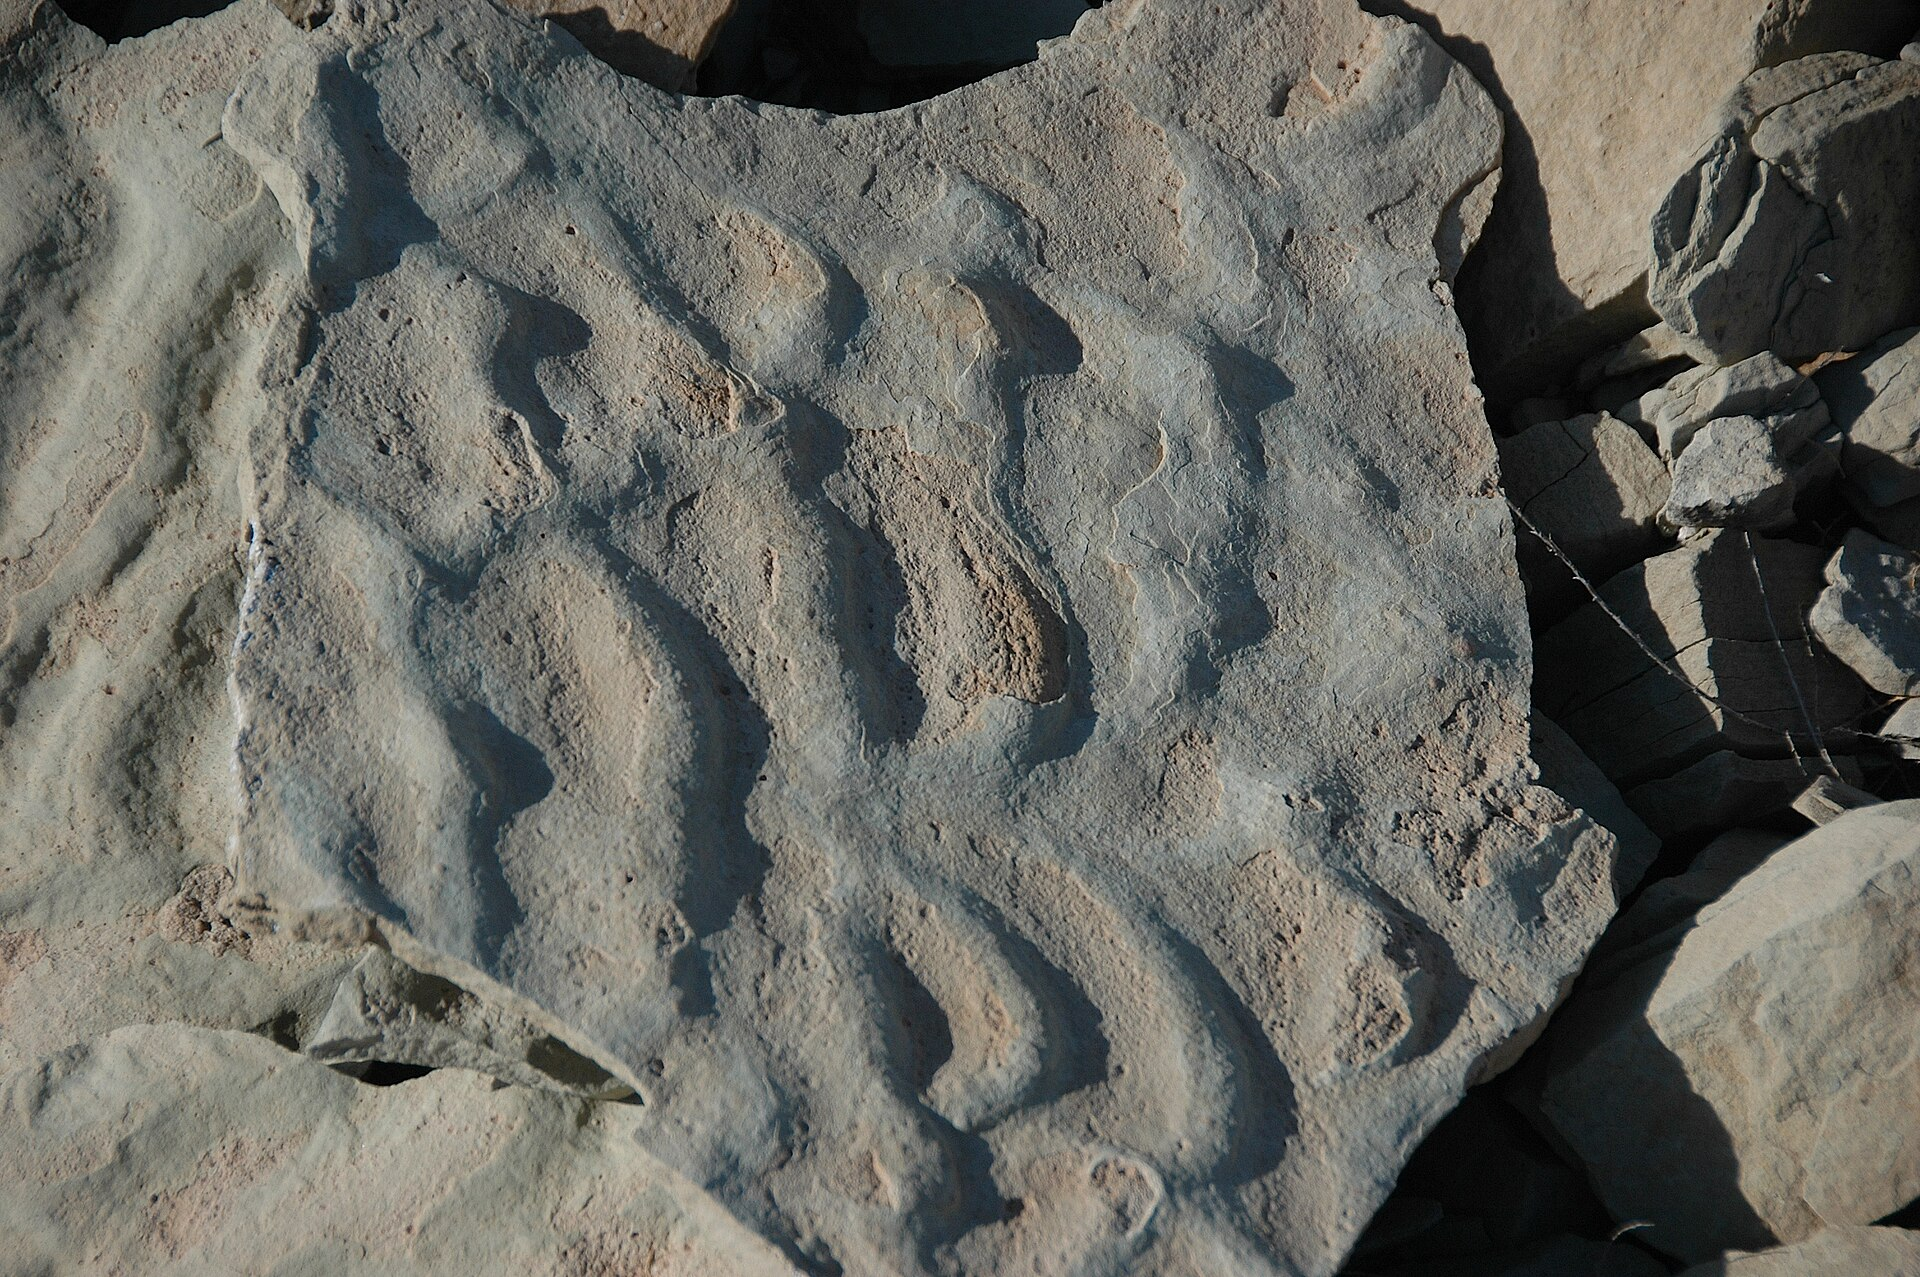
\includegraphics[width=0.56\linewidth]{images/book1/g7-ripple-marks.jpg}

{\small Marcas de ondulação numa laje de arenito no Parque Nacional
Capitol Reef, em Utah (Estados Unidos): a \omterm{def:g3:stones-pebbles-sand:sand}{areia} foi um dia ondulada pela
água em movimento, como a \omterm{def:g3:stones-pebbles-sand:sand}{areia} de uma praia ou do leito de um riacho
hoje. Fotografia: James St.~John (CC BY 2.0, via Wikimedia Commons).}
% ledger: commons:ripples, nps:ripple-marks
\label{fig:g7:sediments-and-fossils:ripples}
\end{omfigure}

\begin{example}[O alto do Grand Canyon]\label{ex:g7:sediments-and-fossils:kaibab}
O Calcário Kaibab, a camada mais alta do Grand Canyon, está cheio de
conchas de braquiópodes e de pedaços de caule de crinoides, dois animais
marinhos. Ele se formou no fundo de um \omterm{def:g2:water-on-earth:ocean}{mar}. Hoje, a mesma camada fica a
até cerca de \qty{2700}{m} (\num{9000}~pés) acima do \omterm{def:g4:world-physical-map:altitude}{nível do mar}: desde
que ela se formou, a região inteira foi levantada.
% ledger: nps:grca-fossils, nps:grca-kaibab
\end{example}

Uma pilha de camadas pode ser desenhada como uma \emph{coluna}: as camadas
empilhadas na ordem em que se formaram, com a sua espessura em escala e as
suas pistas anotadas ao lado. A coluna das Colinas de Varden, a região
inventada dos exercícios desta coleção, está abaixo.

\begin{omfigure}
\begin{tikzpicture}
  \begin{axis}[width=4.2cm, height=9.2cm, scale only axis=false, xmin=0, xmax=1, ymin=-60, ymax=485,
      axis x line=none, axis y line*=left, ytick={0,100,200,300,400},
      ylabel={metros acima da base do arenito}, label style={font=\footnotesize},
      tick label style={font=\scriptsize}, clip=false]
    \addplot[lith schist, draw=black!70, line width=0.3pt] table {figdata/out/grade-7-varden_column-unit-older.dat};
    \addplot[lith sandstone, draw=black!70, line width=0.3pt] table {figdata/out/grade-7-varden_column-unit-sandstone.dat};
    \addplot[lith limestone, draw=black!70, line width=0.3pt] table {figdata/out/grade-7-varden_column-unit-limestone.dat};
    \addplot[lith shale, draw=black!70, line width=0.3pt] table {figdata/out/grade-7-varden_column-unit-shale.dat};
    \addplot[om lith={white}{om limestone}, draw=black!70, line width=0.3pt] table {figdata/out/grade-7-varden_column-unit-chalk.dat};
    \node[anchor=west, align=left, font=\footnotesize] at (axis cs:1.12,450) {\textbf{giz}: o seu topo foi\\desgastado (só a sua base está desenhada)};
    \node[anchor=west, align=left, font=\footnotesize] at (axis cs:1.12,350) {\textbf{folhelho}, \qty{100}{m}: grãos muito finos;\\amonites};
    \node[anchor=west, align=left, font=\footnotesize] at (axis cs:1.12,210) {\textbf{calcário}, \qty{180}{m}:\\corais e conchas};
    \node[anchor=west, align=left, font=\footnotesize] at (axis cs:1.12,60) {\textbf{arenito}, \qty{120}{m}:\\marcas de ondulação, pegadas};
    \node[anchor=west, align=left, font=\footnotesize] at (axis cs:1.12,-30) {rochas mais velhas (xisto e granito),\\aplainadas antes de vir o arenito};
  \end{axis}
\end{tikzpicture}

\medskip
{\small A coluna das Colinas de Varden, a região inventada desta coleção:
as camadas na ordem em que se formaram, a primeira embaixo, com as suas
espessuras em escala. Os \omterm{def:g7:sediments-and-fossils:fossil}{fósseis} e as marcas anotados ao lado são dados
de exercício.}
% ledger: (invented region: figdata/shared/region.py, drawn by figdata/grade-7/varden_column.py)
\label{fig:g7:sediments-and-fossils:column}
\end{omfigure}

\begin{omfigure}
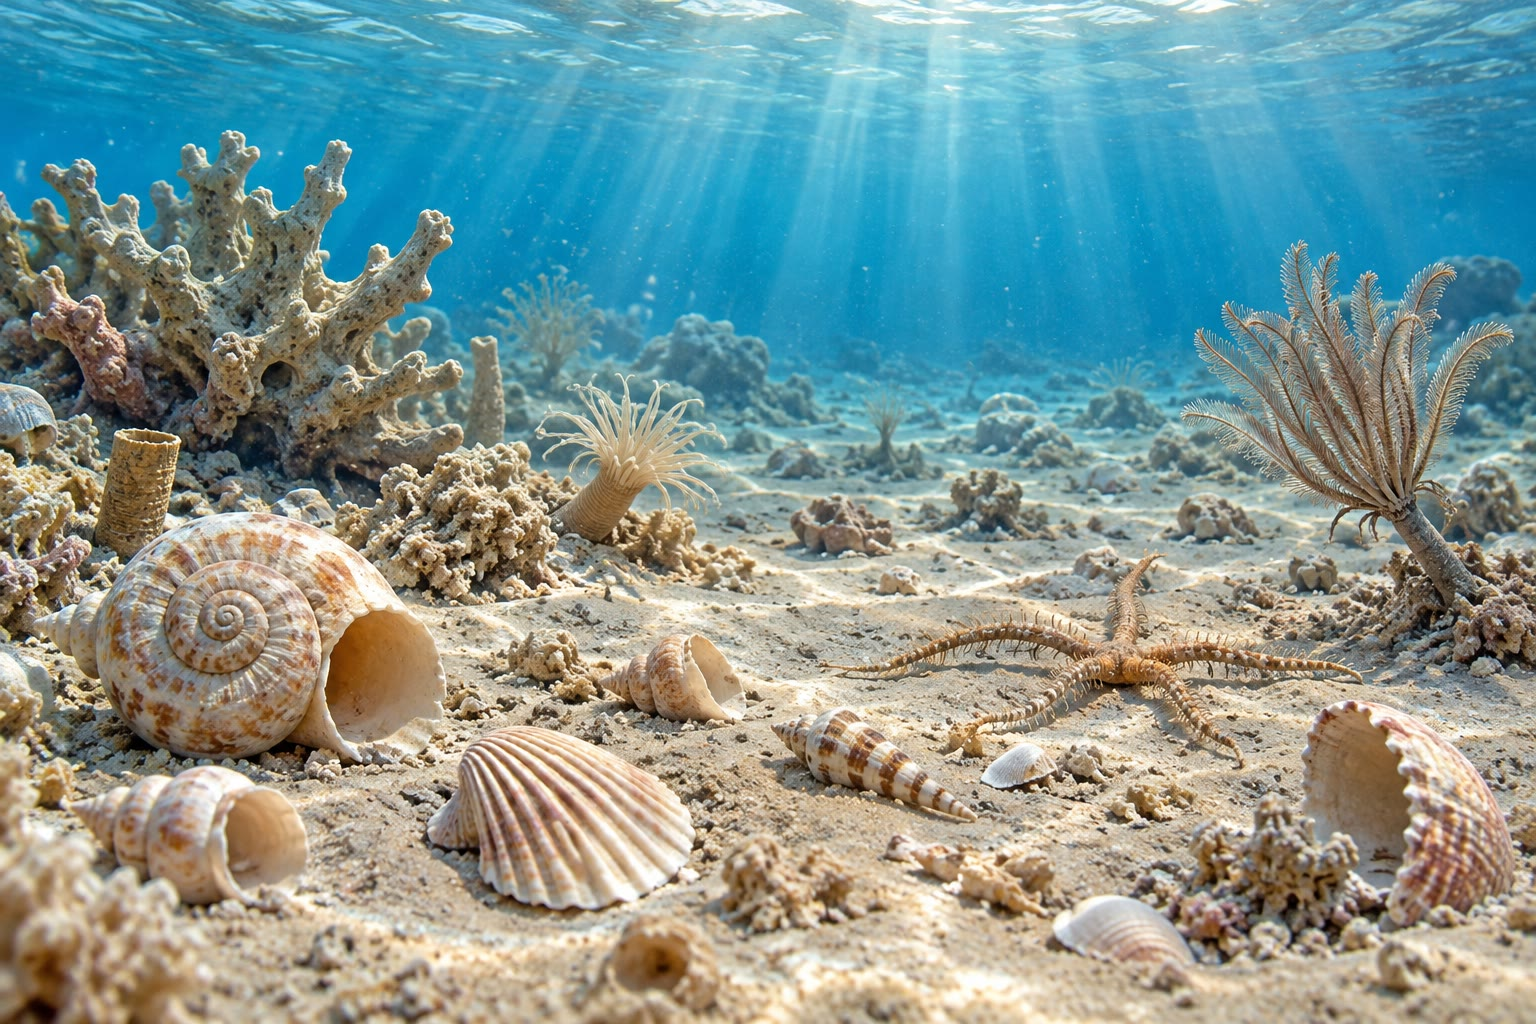
\includegraphics[width=0.6\linewidth]{images/book1/ai/g7-shallow-sea.jpg}

{\small Um fundo de \omterm{def:g2:water-on-earth:ocean}{mar} quente e raso de muito tempo atrás, tal como ele
poderia ser enquanto conchas e pedaços de coral se depositavam num futuro
calcário (ilustração de uma cena genérica feita por IA).}
\label{fig:g7:sediments-and-fossils:shallow-sea}
\end{omfigure}

\begin{remark}[Olhe, fotografe, deixe no lugar]\label{rem:g7:sediments-and-fossils:leave}
Em muitos lugares protegidos, é proibido levar um \omterm{def:g7:sediments-and-fossils:fossil}{fóssil} embora: no Grand
Canyon, por exemplo, a lei proíbe desenterrar, mover ou levar qualquer
\omterm{def:g7:sediments-and-fossils:fossil}{fóssil}. Um visitante que encontra um \omterm{def:g7:sediments-and-fossils:fossil}{fóssil} tira uma fotografia ou faz um
desenho, deixa-o onde está, para os outros verem e para os cientistas
estudarem, e avisa um guarda do parque.
\end{remark}
% ledger: nps:grca-fossils

\begin{inthefield}[Sedimentos que se depositam hoje]
Numa praia, na beira de um \omterm{def:g1:landscapes-around-us:water}{lago} ou na margem de um riacho, com um adulto,
observe a \omterm{def:g3:stones-pebbles-sand:sand}{areia} embaixo da água rasa: a água em movimento a modela em
ondulações, como as que ficaram guardadas no velho arenito. Deixe uma
pegada na \omterm{def:g3:stones-pebbles-sand:sand}{areia} molhada perto da beira da água e observe o que as ondas
seguintes fazem com ela. Depois de um dia de \omterm{def:g4:clouds-rain-snow:precipitation}{chuva}, observe uma poça que
secou: uma película fina de \omterm{def:g3:stones-pebbles-sand:sand}{lama} fina muitas vezes cobre a \omterm{def:g3:stones-pebbles-sand:sand}{areia} do seu
fundo --- os grãos mais finos se depositaram por último, quando a água
estava parada. Desenhe o que você vê, e anote onde e quando.
\end{inthefield}
% ledger: nps:ripple-marks, ucmp:footprints, usgs:strata

\section{Exercícios}

\begin{exercise}[$\star$]\label{exo:g7:sediments-and-fossils:1}
Ligue cada palavra ao seu significado: \omterm{def:g7:sediments-and-fossils:sediment}{sedimento}; \omterm{def:g7:sediments-and-fossils:layer}{estrato}; \omterm{def:g7:sediments-and-fossils:fossil}{fóssil}; \omterm{def:g7:sediments-and-fossils:fossil}{molde};
\omterm{def:g7:sediments-and-fossils:fossil}{contramolde}; \omterm{def:g7:sediments-and-fossils:fossil}{icnofóssil}. (a) Um oco deixado numa \omterm{def:g3:stones-pebbles-sand:rock}{rocha} onde uma concha se
dissolveu. (b) Uma pegada ou uma toca conservada numa \omterm{def:g3:stones-pebbles-sand:rock}{rocha}. (c) Material
solto depositado pela água, pelo vento ou pelo gelo. (d) Uma cópia de
pedra feita quando um oco se enche de \omterm{def:g6:rocks-and-minerals:mineral}{minerais}. (e) Uma lâmina de
\omterm{def:g7:sediments-and-fossils:sediment}{sedimento} depositada de uma só vez. (f) O resto ou o vestígio de um ser
vivo de muito tempo atrás, conservado na \omterm{def:g3:stones-pebbles-sand:rock}{rocha}.
\end{exercise}

\begin{exercise}[$\star$]\label{exo:g7:sediments-and-fossils:2}
Ponha estas etapas em ordem, para contar como uma concha vira um \omterm{def:g7:sediments-and-fossils:fossil}{fóssil}
na superfície: (a) a \omterm{def:g5:water-shapes-the-land:erosion}{erosão} desgasta as camadas de cima; (b) o animal
morre no fundo do \omterm{def:g2:water-on-earth:ocean}{mar}; (c) novas camadas se empilham e a concha vira
pedra; (d) a \omterm{def:g3:stones-pebbles-sand:sand}{lama} cobre a concha depressa.
\end{exercise}

\begin{exercise}[$\star$]\label{exo:g7:sediments-and-fossils:3}
Use a tabela das pistas. Onde cada camada se formou? (a) Um calcário
cheio de corais. (b) Um arenito cuja superfície mostra marcas de
ondulação. (c) Uma camada escura de carvão. (d) Um folhelho com marcas de
folhas e a asa de uma libélula.
\end{exercise}

\begin{exercise}[$\star$]\label{exo:g7:sediments-and-fossils:4}
Verdadeiro ou falso? Corrija as falsas. (a) Todo animal que morre vira
\omterm{def:g7:sediments-and-fossils:fossil}{fóssil} um dia. (b) Uma pegada pode ser um \omterm{def:g7:sediments-and-fossils:fossil}{fóssil}. (c) Quando a água
barrenta desacelera, a \omterm{def:g3:stones-pebbles-sand:sand}{lama} fina se deposita primeiro. (d) Os \omterm{def:g7:sediments-and-fossils:sediment}{sedimentos}
se depositam na horizontal.
\end{exercise}

\begin{exercise}[$\star\star$]\label{exo:g7:sediments-and-fossils:5}
Use a coluna das Colinas de Varden. (a) Dê a espessura do arenito, do
calcário e do folhelho. (b) Qual é a espessura total deles? (c) Que
porcentagem desse total é calcário? Arredonde para o número inteiro mais
próximo. (d) Por que a coluna não dá nenhuma espessura para o giz?
\end{exercise}

\begin{exercise}[$\star\star$]\label{exo:g7:sediments-and-fossils:6}
Uma aluna sacode um pote de água com \omterm{def:g3:stones-pebbles-sand:pebble}{cascalho}, \omterm{def:g3:stones-pebbles-sand:sand}{areia} e \omterm{def:g3:stones-pebbles-sand:sand}{lama}, e o deixa
assentar. (a) Desenhe o pote no dia seguinte e identifique as camadas.
(b) Por que a água ainda está turva depois de uma hora? (c) Ela
acrescenta \omterm{def:g3:stones-pebbles-sand:sand}{areia} e \omterm{def:g3:stones-pebbles-sand:sand}{lama} de novo e deixa assentar. O que ela vê no fundo
agora? (d) Que camada do pote se formou primeiro?
\end{exercise}

\begin{exercise}[$\star\star$]\label{exo:g7:sediments-and-fossils:7}
Qual destes tem mais chance de virar \omterm{def:g7:sediments-and-fossils:fossil}{fóssil}, e qual tem menos? Explique.
(a) Uma água-viva jogada numa praia de pedras. (b) Uma concha de caracol
enterrada na \omterm{def:g3:stones-pebbles-sand:sand}{lama} de um \omterm{def:g1:landscapes-around-us:water}{lago} calmo. (c) Um osso deixado durante anos numa
\omterm{def:g1:landscapes-around-us:landform}{planície} árida. (d) Uma concha de marisco coberta de \omterm{def:g3:stones-pebbles-sand:sand}{areia} numa cheia de
\omterm{def:g1:landscapes-around-us:water}{rio}.
\end{exercise}

\begin{exercise}[$\star\star$]\label{exo:g7:sediments-and-fossils:8}
Uma concha é enterrada numa \omterm{def:g3:stones-pebbles-sand:sand}{areia} que vira arenito. A água que se
infiltra pela \omterm{def:g3:stones-pebbles-sand:rock}{rocha} dissolve a concha completamente. (a) O que sobra na
\omterm{def:g3:stones-pebbles-sand:rock}{rocha}? (b) Depois, \omterm{def:g6:rocks-and-minerals:mineral}{minerais} preenchem esse oco. O que se forma? (c) A
própria concha ainda está lá? (d) Por que se encontram \omterm{def:g7:sediments-and-fossils:fossil}{moldes} e
\omterm{def:g7:sediments-and-fossils:fossil}{contramoldes} mais vezes no arenito que no folhelho? (Pense em quão
facilmente a água passa entre os grãos.)
\end{exercise}

\begin{exercise}[$\star\star$]\label{exo:g7:sediments-and-fossils:9}
O Grand Canyon tem em média \qty{1.6}{km} de profundidade. (a) Escreva
essa profundidade em metros. (b) Suponha que as paredes do cânion fossem
feitas de camadas de \qty{80}{m} de espessura cada uma: quantas camadas
caberiam da borda até o fundo? (c) Uma camada de \qty{160}{m} é que
porcentagem da profundidade?
\end{exercise}

\begin{exercise}[$\star\star$]\label{exo:g7:sediments-and-fossils:10}
Encontram-se pegadas de dinossauros num arenito. (a) Os dinossauros
andavam sobre \omterm{def:g3:stones-pebbles-sand:rock}{rocha} dura? Explique. (b) Por que a maioria das pegadas
deixadas numa praia lamacenta desaparece? (c) O que precisou acontecer
logo depois da passagem dos dinossauros para que as pegadas fossem
conservadas? (d) Uma pegada é um \omterm{def:g7:sediments-and-fossils:fossil}{fóssil} do corpo ou um \omterm{def:g7:sediments-and-fossils:fossil}{icnofóssil}?
\end{exercise}

\begin{exercise}[$\star\star\star$]\label{exo:g7:sediments-and-fossils:11}
Num \omterm{def:g1:landscapes-around-us:water}{lago}, cada cheia deixa uma camada de \omterm{def:g3:stones-pebbles-sand:sand}{areia} de cerca de \qty{2}{cm} de
espessura, e as semanas calmas que vêm depois, uma camada de \omterm{def:g3:stones-pebbles-sand:sand}{lama} de
cerca de \qty{5}{mm} (dados de exercício). (a) Qual é a espessura, em
milímetros, de um par de camadas? (b) Um testemunho tirado do fundo do
\omterm{def:g1:landscapes-around-us:water}{lago} tem \qty{1}{m} de comprimento e é feito só desses pares. Quantas
cheias ele registra? (c) Perto da \omterm{def:g5:water-shapes-the-land:source-mouth}{foz} do \omterm{def:g1:landscapes-around-us:water}{rio}, as camadas de \omterm{def:g3:stones-pebbles-sand:sand}{areia} são
mais grossas; longe dela, são mais finas. Explique por quê. (d) Por que
há mais \omterm{def:g3:stones-pebbles-sand:sand}{lama} que \omterm{def:g3:stones-pebbles-sand:sand}{areia} longe da \omterm{def:g5:water-shapes-the-land:source-mouth}{foz}?
\end{exercise}

\begin{exercise}[$\star\star\star$]\label{exo:g7:sediments-and-fossils:12}
Os \omterm{def:g7:sediments-and-fossils:fossil}{fósseis} encontrados nas \omterm{def:g3:stones-pebbles-sand:rock}{rochas} são sobretudo conchas e restos
minúsculos; os \omterm{def:g7:sediments-and-fossils:fossil}{fósseis} de animais moles são raros, e os dinossauros são só
uma parte muito pequena de todos os \omterm{def:g7:sediments-and-fossils:fossil}{fósseis}. (a) Explique por que as
conchas são tão comuns. (b) Explique por que os animais moles são raros.
(c) Uma cientista quer conhecer todos os animais que viviam num \omterm{def:g2:water-on-earth:ocean}{mar}
antigo. Os \omterm{def:g7:sediments-and-fossils:fossil}{fósseis} podem dar a lista completa? Explique.
\end{exercise}

\section{Problema: A coluna das Colinas de Varden}

\begin{problem}[{Problema de fim de semana --- as camadas das Colinas de
Varden são lidas uma por uma, os seus fósseis contam onde elas se
formaram, e calcula-se o tempo necessário para empilhar o calcário}]
\label{pb:g7:sediments-and-fossils:1}
% ledger: (invented region: figdata/shared/region.py; rates are exercise data, figdata/grade-7/varden_column.py part rates)
Use a coluna das Colinas de Varden deste capítulo. O seu arenito mostra
marcas de ondulação e pegadas; o seu calcário guarda corais e conchas; o
seu folhelho é feito de grãos muito finos, com amonites; o giz do alto
foi em parte desgastado.

\medskip
\noindent\textbf{Parte I --- Ler as camadas.}\par\nopagebreak
\begin{enumerate}[beginpenalty=10000]
  \item Liste as quatro camadas, da primeira depositada até a última.
  \item Dê a espessura do arenito, do calcário e do folhelho, e o total
        delas.
  \item Que porcentagem desse total é calcário?
  \item Por que ninguém consegue dizer qual era a espessura do giz quando
        ele se formou?
\end{enumerate}

\medskip
\noindent\textbf{Parte II --- Os fósseis que elas guardam.}\par\nopagebreak
\begin{enumerate}[resume, beginpenalty=10000]
  \item Onde se formou o arenito? Dê duas pistas.
  \item Onde se formou o calcário? Dê a pista.
  \item O folhelho é feito de grãos muito finos. A água estava calma ou em
        movimento quando ele se depositou? Explique.
  \item Conte a história do lugar em três frases, do arenito até o
        folhelho.
\end{enumerate}

\medskip
\noindent\textbf{Parte III --- Quanto tempo levou.}\par\nopagebreak
\begin{enumerate}[resume, beginpenalty=10000]
  \item Escreva a espessura do calcário em centímetros.
  \item Suponha que o arenito se empilhou à razão de \qty{1}{cm} a cada 20
        anos. Quantos anos levaram os seus \qty{120}{m}?
  \item Suponha que o calcário se empilhou à razão de \qty{1}{cm} a cada
        100 anos. Quantos anos levou \qty{1}{m} de calcário?
  \item Quantos anos levaram os \qty{180}{m} de calcário? Quantas vezes
        mais que o arenito isso dá?
\end{enumerate}
\end{problem}
